\documentclass{report}
\usepackage[T1]{fontenc}
\usepackage{color}
\usepackage{amssymb}
\usepackage{amsmath}
\usepackage{eurosym}
\usepackage{graphicx}
\usepackage{textcomp}
\usepackage{listings}
\usepackage{epigraph}
\usepackage{setspace}
\usepackage[some]{background}
\usepackage{gensymb}
\usepackage{tikz}
\usepackage{geometry}
\usepackage{fancyhdr}
\usepackage[english]{babel}
\lstdefinelanguage{scala}{
morekeywords={%
abstract,case,catch,class,def,do,else,extends,%
false,final,finally,for,forSome,if,implicit,import,lazy,%
match,new,null,object,override,package,private,protected,%
return,sealed,super,this,throw,trait,true,try,type,%
val,var,while,with,yield},
otherkeywords={=>,<-,<\%,<:,>:,\#,@},
sensitive=true,
morecomment=[l]{//},
morecomment=[n]{/*}{*/},
morestring=[b]",
morestring=[b]',
morestring=[b]"""
}[keywords,comments,strings]

\lstset{
float=hbp,
language=scala,
basicstyle=\ttfamily\small\color{colBasic},
upquote=true,
aboveskip={1.5\baselineskip},
columns=fullflexible,
showstringspaces=false,
extendedchars=true,
breaklines=true,
showtabs=false,
showspaces=false,
frame=trbl, 
tabsize=4,
numbers=left,
breakautoindent=true,
extendedchars=true,
showstringspaces=false,
identifierstyle=\ttfamily,
frameround=ffff,
captionpos=b,
xrightmargin=0cm,
xleftmargin=0cm,
backgroundcolor=\color{colBackground},
keywordstyle=\bf\color{colKeyword},
commentstyle=\color{colComment},
identifierstyle=\color{colIdent}, 
stringstyle=\color{colString},}\definecolor{colBasic}{rgb}{0.5,0.5,0.8}
\definecolor{colKeyword}{rgb}{0.4,0.5,1}
\definecolor{colBackground}{rgb}{0.1,0.1,0.2}
\definecolor{colComment}{rgb}{0.4,0.4,0.4}
\definecolor{colString}{rgb}{0.8,0.8,0.8}
\definecolor{colIdent}{rgb}{0,0.8,0.8}


\begin{document}
\renewcommand{\chaptername}{Part}
\renewcommand{\thechapter}{\Roman{chapter}}

%\usepackage{lmodern}
%\usepackage{xspace}
%\usepackage{hyperref}
%\usepackage{fancyhdr}

% header style
\pagestyle{fancy}
\renewcommand{\headrulewidth}{1pt}
\fancyhead[L]{February 16th, 2015}
\fancyhead[R]{\textbf{Reference :} model-checking.test-strategy - Version 1}

% Redefine the plain page style
\fancypagestyle{plain}{%
  \fancyhf{}%
  \renewcommand{\headrulewidth}{1pt}
  \fancyhead[L]{February 16th, 2015}
  \fancyhead[R]{\textbf{Reference :} model-checking.test-strategy - Version 1}
  \fancyfoot[C]{\thepage}
}

% title page
\definecolor{sup_strip_color}{rgb}{0.70,0.70,0.70}
\definecolor{inf_strip_color}{rgb}{0.00,0.00,0.00}

\DeclareFixedFont{\bigsf}{T1}{phv}{b}{n}{0.9cm}

\makeatletter                       
\def\printauthor{%                  
    {{\large \@author}}}              
\makeatother

\author{Sofia \textsc{Boutahar} ~\\ David \textsc{Courtinot}}

\begin{titlepage}

\newgeometry{left=1cm,right=4cm,bottom=0cm}
\begin{tikzpicture}[overlay,remember picture]
% the black stripe with the title
\node[
  fill=inf_strip_color,
  anchor=north west,
  text width=\paperwidth,
  text height=2cm,
  text depth=2cm,
  inner xsep=1cm,
  font=\color{white}\bigsf 
  ] 
 at ([yshift=-2.5cm]current page.north west) (blackrect) {Test strategy - Version 1};
% the khaki stripe
\path[fill=sup_strip_color] 
  (blackrect.north west) rectangle ++(\paperwidth,2.5cm);
\end{tikzpicture}

\vspace*{4.5cm}

\noindent
\begin{minipage}{0.35\linewidth}
    \begin{flushright}
        \printauthor
    \end{flushright}
\end{minipage} \hspace{15pt}
%
\begin{minipage}{0.02\linewidth}
    \rule{1pt}{175pt}
\end{minipage} \hspace{-10pt}
%
\begin{minipage}{0.6\linewidth}
\vspace{5pt}
\newenvironment{test}{\begin{center}}{\end{center}}
\hspace{10pt}
\begin{minipage}{\linewidth} 
\textbf{Reference :} model-checking.test-strategy ~\\
February 16th, 2015
\end{minipage}
\end{minipage}

\vspace{8cm}
\begin{minipage}{0.20\linewidth}
    \begin{flushright}
       
        \begin{tabular}{ll}
	 \textit{Signatures} & \\
			& \textbf{Project manager - Zohour \textsc{Abouakil} :} \\
            & \textbf{Quality responsible - David \textsc{Courtinot} :} \\
            & \textbf{Customers - David \textsc{Doose} - Julien \textsc{Brunel} :} \\
        \end{tabular}
    \end{flushright}
\end{minipage}

\end{titlepage}
\restoregeometry
\tableofcontents
\newgeometry{left=2.1cm,right=2.1cm}
\chapter{Overview}

\paragraph{}
\hspace{4mm}The purpose of a test strategy is to clarify the major tasks and challenges of the test project, define what we want to accomplish and how we are going to achieve it. Moreover, it helps us figure out if there are missing requirements in the project and have a clear state of it at any point.
Our project is divided into two parts: The conversion of the AST to the CFG and the model checking using CTL.
The first part can be divided into two subparts : Parsing the file generated by the Clang compiler and converting the AST to the CFG.

\chapter{Testing AST conversion to CFG}

\section{Test strategy}

\paragraph{}
\hspace{4mm}When we identify a particular problem in our code, we try to debug it and the fix the issues. 
To make sure that the fix works, we test our program again to see if it works. Therefore, it is not sufficient to validate the test if the tested program works, we should make sure that our fixes don't create some other problems in any other parts of our projects due to dependencies.
So, a set of related test cases may have to be repeated again, to make sure that nothing else is affected our fixes.
Basically, whenever there is a fix in one unit, we repeat all unit test cases for that unit in order to achieve a higher level of abstraction and quality.

\section{Testing the parser}

\paragraph{}
\hspace{4mm}The clang compiler takes a C++ source code as input 
and returns a file describing an Abstract Syntax Tree. The purpose of creating a parser
is to extract from the Clang file all the useful information and build a tree
that contains it.

\paragraph{}
\hspace{4mm}As the number of possible tests for our parser is practically infinite, we created several tests
starting from the easiest to the most complicated one. The aim was to ensure that our
program is working for the minimum number of tests needed to get the coverage we want.

\begin{center}
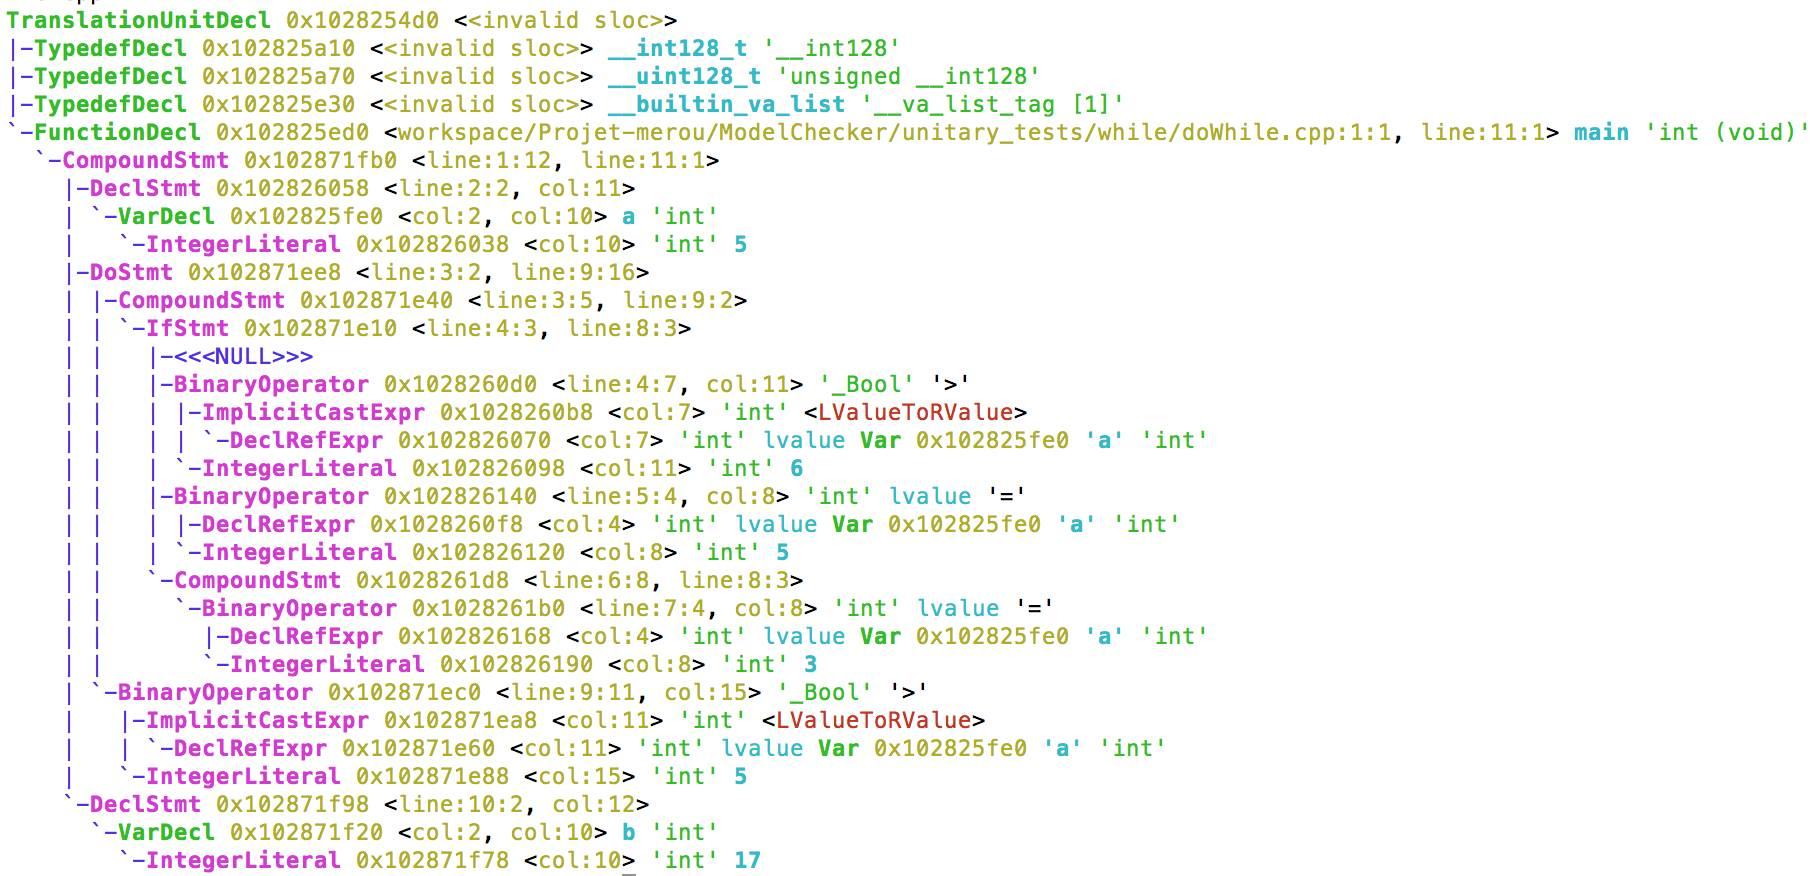
\includegraphics[scale=0.3]{data/dowhile_clang.jpg}
~\\~\\Figure II.1 - Example of an input AST (generated automatically thanks to Clang by our test program) of a do-while statement
\end{center}

\begin{center}
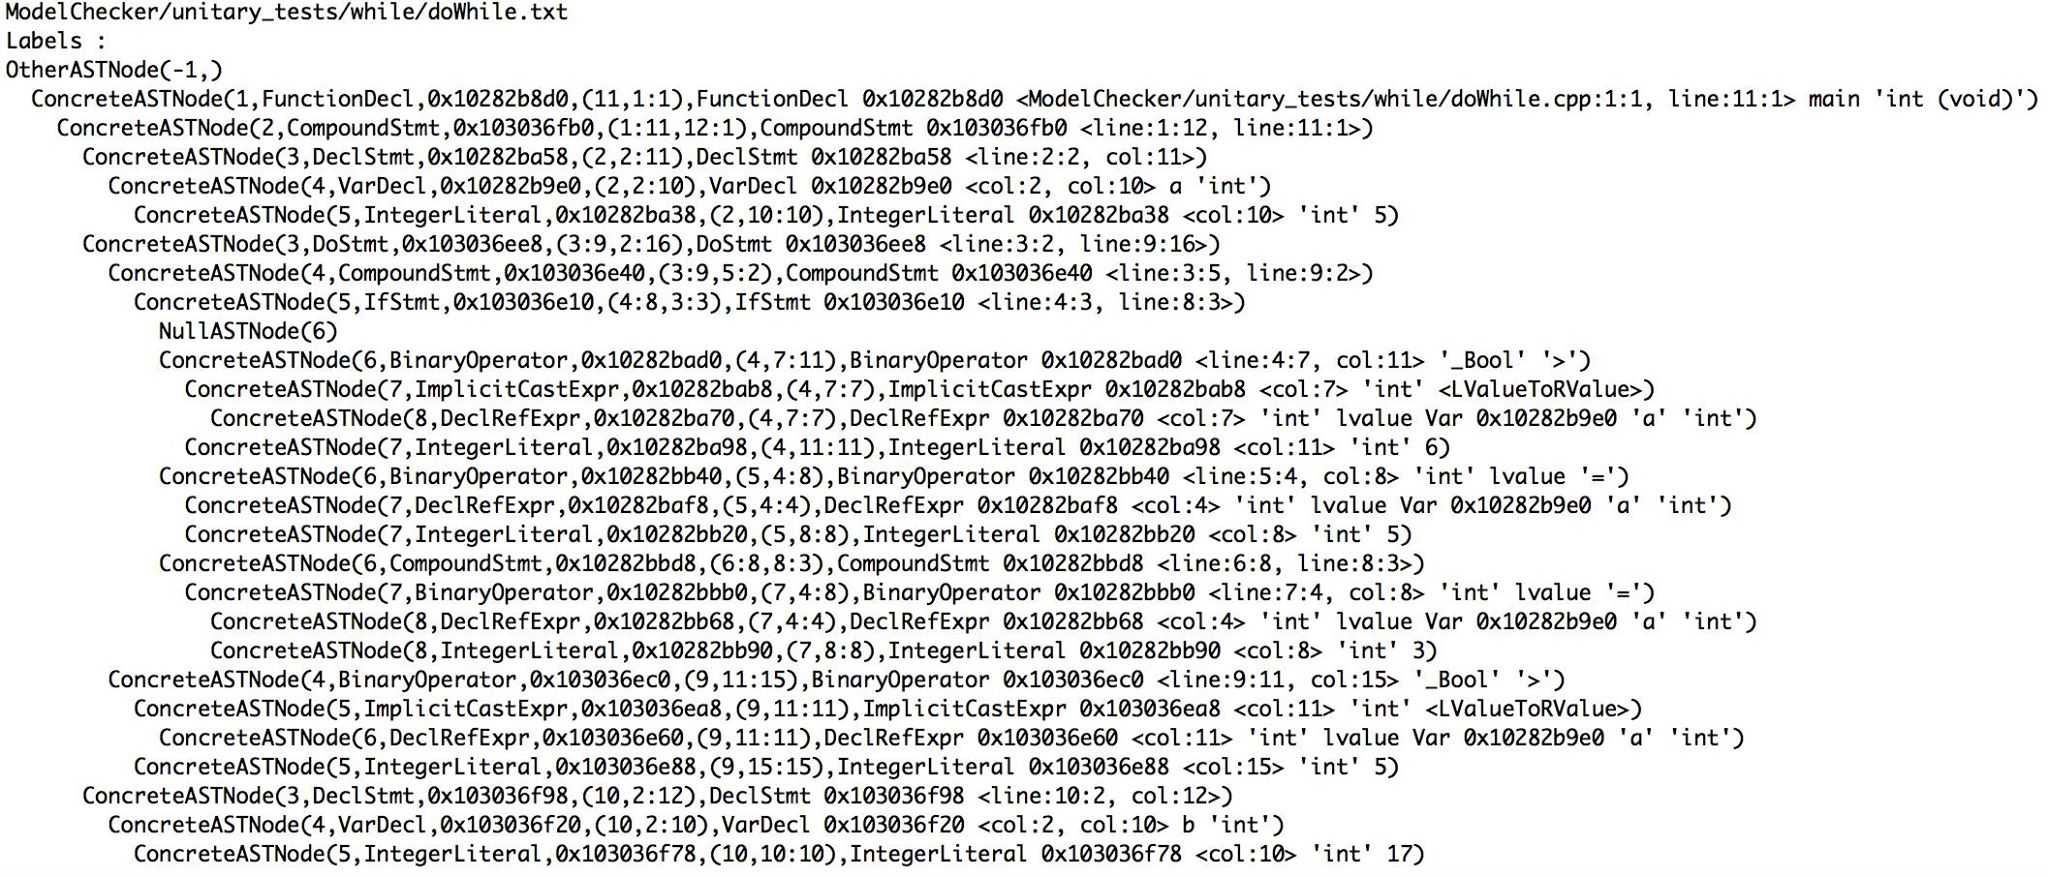
\includegraphics[scale=0.3]{data/while_astNode.jpg}
~\\~\\Figure II.2 - Corresponding output (ASTNode tree data-structure), as the test program prints it
\end{center}

\section{Testing results}

\paragraph{}
\hspace{4mm}We

\chapter{Testing the model checking algorithm}

\paragraph{}
\hspace{4mm}Unlike the CFG part, there is a lot of room here for automated tests because there are many elementary operations that must return a specific result. We have written some generic methods 
that enable to automatically check the output rather than performing a manual check. This constitutes a very simple 
testing framework that we will present here. We will then present our process and results for the first iteration.

\section{Automated testing}

\paragraph{}
\hspace{4mm}All the test functions rely on generic methods such as \textbf{assertEquals} or \textbf{assertTrue} that print
the result of the test with its number. This way, it is fairly easy to generate a log file and get the result of the tests
in the clearest way. You can find below an example of such test functions :

\begin{lstlisting}[language=scala
]
def printMsg(failed: Boolean) = { 
        val msg = "\tTest %d %s".format(i,if (failed) "failed" else "passed") 
        if (failed) Console.err.println(msg)
        else        println(msg)
        i += 1
}
def assertEquals[T](t0: T, t1: T) = printMsg(t0 != t1)
def assertTrue(b: Boolean)       = printMsg(!b)
def compareEnv[T](envT1: Env[T], envT2: Env[T], expected: Env[T]) = assertEquals(envT1 interEnv envT2,    def testNeg[T](env: Env[T], envs: Env[T]*)  = assertEquals(!env,Set(envs: _*))
\end{lstlisting}
\section{Testing process}

\paragraph{}
\hspace{4mm}For this part, we have made a lot of unitary tests. We first tested every operation defined on the Environment subclasses
because it constitutes the base of almost all computations performed by the algorithm. Once we were assured that these operations were correctly implemented,
we tested the operations of the ModelChecker, starting with the elementary operations to the compound operations. We still have not tested
the highest level functions.

\section{Results}

\paragraph{}
\hspace{4mm}We detected and fixed some minor bugs in our elementary operations.  Globally, all the functions were implemented correctly.
Note that we had to rewrite those tests when we changed our conception for the CTL part. This was fairly easy thanks to the good structure of the code and we soon
obtained similar results. Just as an example, here is an example of the log generated by the automated tests.

\begin{center}
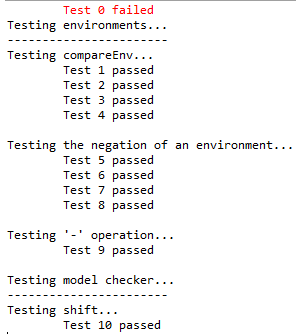
\includegraphics[scale=0.7]{data/test-log.png}
~\\~\\Figure III.1 - Example of a test log file
\end{center}

\end{document}
